\documentclass[conference]{IEEEtran}

\usepackage{cite}
\usepackage[pdftex]{graphicx}
% declare the path(s) where your graphic files are
\graphicspath{{images/}}
\usepackage[cmex10]{amsmath}
\usepackage{algorithmic}
%\usepackage{array}
\usepackage[caption=false,font=footnotesize]{subfig}
\usepackage{stfloats}
\usepackage{url}
\usepackage[utf8]{inputenc}
\usepackage{multirow}
\usepackage{booktabs}
\usepackage{tabularx}

% correct bad hyphenation here
\hyphenation{op-tical net-works semi-conduc-tor}

\begin{document}

\title{Automatic Mobile Video Director}

\author{
	\IEEEauthorblockN{Alexander Egurnov}
	\IEEEauthorblockA{University of Mannheim\\
		aegurnov@mail.uni-mannheim.de}
\and
	\IEEEauthorblockN{Thilo Weigold}
	\IEEEauthorblockA{University of Mannheim\\
		tweigold@mail.uni-mannheim.de}
\and
	\IEEEauthorblockN{Jon Pettersen}
	\IEEEauthorblockA{University of Oslo\\
		jonup@student.matnat.uio.no}
\and
	\IEEEauthorblockN{Alf-André Walla}
	\IEEEauthorblockA{University of Oslo\\
		alfandrw@ifi.uio.no}
}

% This a recommended way to give more than 3 authors but it looks ugly.
% Default author block above still fits in one line.
%\author{
	%\IEEEauthorblockN{
		%Alexander Egurnov\IEEEauthorrefmark{1},
		%Thilo Weigold\IEEEauthorrefmark{2},
		%Jon Pettersen\IEEEauthorrefmark{3}, 
		%Alf-André Walla\IEEEauthorrefmark{4}
	%}
	%\IEEEauthorblockA{
		%\IEEEauthorrefmark{1}University of Mannheim\\
		%aegurnov@mail.uni-mannheim.de
	%}
	%\IEEEauthorblockA{
		%\IEEEauthorrefmark{2}University of Mannheim\\
		%tweigold@mail.uni-mannheim.de
	%}
	%\IEEEauthorblockA{
		%\IEEEauthorrefmark{3}University of Oslo\\
		%jonup@student.matnat.uio.no
	%}
	%\IEEEauthorblockA{
		%\IEEEauthorrefmark{4}University of Oslo\\
		%alfandrw@ifi.uio.no
	%}
%}

\maketitle

\begin{abstract}
The abstract goes here.

WRITE ME !!!!!!!!!!!!!!!!!!!!!!!!!!!!!!!!!!!!!
WRITE ME !!!!!!!!!!!!!!!!!!!!!!!!!!!!!!!!!!!!!
WRITE ME !!!!!!!!!!!!!!!!!!!!!!!!!!!!!!!!!!!!!
WRITE ME !!!!!!!!!!!!!!!!!!!!!!!!!!!!!!!!!!!!!
WRITE ME !!!!!!!!!!!!!!!!!!!!!!!!!!!!!!!!!!!!!
WRITE ME !!!!!!!!!!!!!!!!!!!!!!!!!!!!!!!!!!!!!
WRITE ME !!!!!!!!!!!!!!!!!!!!!!!!!!!!!!!!!!!!!
WRITE ME !!!!!!!!!!!!!!!!!!!!!!!!!!!!!!!!!!!!!
WRITE ME !!!!!!!!!!!!!!!!!!!!!!!!!!!!!!!!!!!!!

\end{abstract}

\section{Introduction}

% TODO more like in the last 10 years
In the recent years the Internet has changed a lot. 
It is not about retrieving simple HTML pages from websites anymore, 
but rather sharing news, videos and pictures from all over the world.
With the advent of the ``Web 2.0'' user-generated content has become a crucial part of the Internet we know nowadays.
% TODO It would be nice to have a link to some kind of report comparing multimedia/web2.0 traffic
Being social is another rather important need of an average internet user.
Well-known platforms like YouTube, Twitch, Facebook, Twitter, Instagram, Flickr and many other
make it easy for everyone to share their thoughts in a vast variety of multimedia formats.

A considerable contribution to changing the web is done by changing how people typically access it.
In the past the main role of mobile phones was one-to-one communication. 
But as the technology evolved, such devices gradually assumed functions of fully capable handheld computers.
As all the necessary operations to shoot, process and publish a complex multimedia file moved to a single device, 
the amount of user-generated content experienced an explosive growth.
% TODO link to proof
Due to more precise sensors, integrated high-resolution cameras and, of course, faster mobile networking technologies, 
it has never been as simple to share content from any place and at any time.
The ubiquitous use of mobile phones leads to completely new challenges and opportunities for web services 
that use user data in order to create dynamic content.

There are so many different events happening at the same time, 
that it is easy imagine an interesting public event like a political speech, 
a concert or a sports event which is not covered by professional journalists, photo and video operators.
Fortunately, it has become quite common for spectators to capture parts of ongoing events on their portable gadgets' cameras.
Such videos are rarely organized in any reasonable manner, except for user-provided descriptions and hashtags, 
which are often abused and give little idea of the content's quality.

The potential being wasted here is tremendous. 
One obvious application for these videos is providing a near real-time media coverage of the event for internet viewers.
However, if every video is uploaded right from the venue, an excessively high bandwidth will be consumed.
But due to a vast variety of portable devices and dispersion of filming abilities of their owners,
to create of a high quality mash up of an event some elaborate selection mechanism is needed.

In this paper we attempt to build a system, called Automatic Mobile Video Director, capable of dealing with this kind of situations.
We henceforth focus on implementing interactions between multiple clients and one central server, the automatic video director,
keeping in mind bandwidth and computational complexity problems, which were mentioned above. 
As a mean of limiting the amount of data transmitted by each mobile device during the event we only require 
that some textual metadata, which is based on sensor data as well as general video parameters, is sent to the server.
The server then makes a decisions whether each particular video is worth uploading directly from the venue
and dispatches commands to clients to start uploading.
We give only a brief overview and a very basic implementation of sensor data processing as this area of research 
is being studied by another group. The same applies to the selection criteria of the director algorithm.

% An example of a floating figure using the graphicx package.
% Note that \label must occur AFTER (or within) \caption.
% For figures, \caption should occur after the \includegraphics.
% Note that IEEEtran v1.7 and later has special internal code that
% is designed to preserve the operation of \label within \caption
% even when the captionsoff option is in effect. However, because
% of issues like this, it may be the safest practice to put all your
% \label just after \caption rather than within \caption{}.
%
% Reminder: the "draftcls" or "draftclsnofoot", not "draft", class
% option should be used if it is desired that the figures are to be
% displayed while in draft mode.
%
%\begin{figure}[!t]
%\centering
%\includegraphics[width=2.5in]{myfigure}
% where an .eps filename suffix will be assumed under latex, 
% and a .pdf suffix will be assumed for pdflatex; or what has been declared
% via \DeclareGraphicsExtensions.
%\caption{Simulation Results.}
%\label{fig_sim}
%\end{figure}

% Note that IEEE typically puts floats only at the top, even when this
% results in a large percentage of a column being occupied by floats.
% However, the Computer Society has been known to put floats at the bottom.

% An example of a double column floating figure using two subfigures.
% (The subfig.sty package must be loaded for this to work.)
% The subfigure \label commands are set within each subfloat command,
% and the \label for the overall figure must come after \caption.
% \hfil is used as a separator to get equal spacing.
% Watch out that the combined width of all the subfigures on a 
% line do not exceed the text width or a line break will occur.
%
%\begin{figure*}[!t]
%\centering
%\subfloat[Case I]{\includegraphics[width=2.5in]{box}%
%\label{fig_first_case}}
%\hfil
%\subfloat[Case II]{\includegraphics[width=2.5in]{box}%
%\label{fig_second_case}}
%\caption{Simulation results.}
%\label{fig_sim}
%\end{figure*}
%
% Note that often IEEE papers with subfigures do not employ subfigure
% captions (using the optional argument to \subfloat[]), but instead will
% reference/describe all of them (a), (b), etc., within the main caption.

% An example of a floating table. Note that, for IEEE style tables, the 
% \caption command should come BEFORE the table. Table text will default to
% \footnotesize as IEEE normally uses this smaller font for tables.
% The \label must come after \caption as always.
%
%\begin{table}[!t]
%% increase table row spacing, adjust to taste
%\renewcommand{\arraystretch}{1.3}
% if using array.sty, it might be a good idea to tweak the value of
% \extrarowheight as needed to properly center the text within the cells
%\caption{An Example of a Table}
%\label{table_example}
%\centering
%% Some packages, such as MDW tools, offer better commands for making tables
%% than the plain LaTeX2e tabular which is used here.
%\begin{tabular}{|c||c|}
%\hline
%One & Two\\
%\hline
%Three & Four\\
%\hline
%\end{tabular}
%\end{table}

% Note that IEEE does not put floats in the very first column - or typically
% anywhere on the first page for that matter. Also, in-text middle ("here")
% positioning is not used. Most IEEE journals use top floats exclusively.
% However, Computer Society journals sometimes do use bottom floats - bear
% this in mind when choosing appropriate optional arguments for the
% figure/table environments.

\section{Related work}

As mentioned above, public interest to capturing and sharing videos from public events has increased 
with the introduction of mobile devices with high resolution cameras and wireless internet connection.
Quite obviously, it entailed an increase in the number of research projects trying to make these tasks easier 
and to reduce the strain of uploading of such videos by hand.

One possible approach is discussed in \cite{engstrom_mobile_2012}.
It proposes a way of making videos where five people are able to set up a connection between their mobile devices,
assign roles to each device, one of them being assigned the role of director and the others are cameramen,
and capture an event from different perspectives. Video selection is performed manually by the designated person.

Another paper \cite{shrestha_automatic_2010} focuses on devising an algorithm which would create 
a ``mashup'' of several video and audio streams automatically.
More attention is paid to satisfying a formal model of a perfect video, 
and selection of video streams is solved as an optimization problem.
However their approach requires all video files to be present when the algorithm works, 
as it first needs to synchronize them and run image analysis.

In case of live streaming the former approach would require an overwhelming amount of data to be transmitted.
The paper \cite{seshadri_demand_2014} proposes a method of reducing data traffic significantly.
They achieve it through the use of metadata captured by all kinds of sensors which are present on modern handheld devices.
The metadata helps to evaluate quality of videos prior to uploading them from client devices on the event venue to the server.
This way only the best videos actually get uploaded and consume traffic.
As it is pointed out in the paper, this is a huge issue for some extremely popular events like USA's SuperBowl \cite{Erman:2013}.

Systems like the ones discussed above can be used to generate a summary of an event by fusing parts of different video clips together.
However, to discover exactly when a video is shot also represents a challenge. 
Failing to find the exact time a video is shot may lead to videos overlapping or failing to cover the entire event 
by leaving gaps in the video timeline \cite{shrestha_automatic_2010}. 
An approach leveraged in \cite{jain_focus:_2013} is to use GPS to extract timestamps. 
Another way to addresses this issue is by using the audio in the video files 
to generate a unified timeline of the event \cite{shrestha_automatic_2010}. 

A different issue is identifying a region of interest or point of interest.
These terms describe areas of the event that are more interesting than others. 
We probably will find a video of a concert more interesting if the camera is pointing towards the stage than one pointing somewhere else.
Several solutions have been proposed for solving this problem.
One of them is to go through frames of the video to see if they resemble the main attraction of the event, 
i.e. a stage on a concert, or the singer on that stage. 
However the reliance on the sensors in the mobile devices for discovering such regions seems to be a more preferable method.
\cite{cricri_sensor-based_2012} uses the built-in compass found on mobile devices to make sure 
that the camera is pointing in the right direction.
Their system also uses compass to detect when camera changes direction. 
An assumption is made that if operator suddenly turns his or her camera in some direction,
there is a chance that something interesting is happening there.

When it comes to detecting what is pictured in a video, one might also want to identify the activity which was filmed.
This can be used to relieve managers of such systems from the trouble of marking each video with appropriate tags. 
Authors of \cite{cricri_sport_2014} have created a system that is capable of detecting which of several kinds of sport is being filmed.

Another issue is when to start recording and how to define what is an event.
In the paper \cite{bao_movi:_2010} a system is described which can detect when a social event is taking place, leveraging
mobile devices sensors and communication between nearby devices.
The devices then start recording and ultimately a ``highlights'' video coverage is created.
Among other things, authors use the sound of laughter to trigger event detection.

% TODO Design?
\section{Methodology}

\subsection{System Overview}
In this section we give a brief overview of the whole system.
Detailed discussions of our implementation will follow in the subsections afterwards. 
To implement our idea of an Automatic Mobile Video Director it was necessary to find the right structural organization for our system.
Given requirements and logical distribution of tasks leads us to the decision 
to implement our service in a conventional client-server architecture.
Figure~\ref{fig:gen_arch} shows our general system architecture, consisting of multiple clients and one central server.

This architectural set up entails some important advantages.
Client-Server design gives us opportunity to strictly separate tasks and work between clients and server.
Compared to other possible architectures, like peer to peer, we are able to centralize all resources
and important computation in one place. 
Resources, like battery and computational effort can be saved on the client side, 
while computationally intensive tasks are carried out on the server side. 
In peer to peer networks clients would have to communicate with each other, 
which would produce big communication overhead to weight of important resources.
However, these resources are limited and needed for recording videos and sending them upon request to our central Video Director.
Therefore we believe that the client-server architecture best matches our requirements.


The server set up uses local file system for video storage, a MySQL database for storing and retrieving meta data persistently and a RESTful interface to handle HTTP requests and responses.
Additional core function is the director algorithm which is used to make decisions about which video clients should upload.
Nginx web server is used to stream resulting video from our web server to viewers.
This feature is not fully implemented yet and left for future work and improvements.
Detailed descriptions of our server and client implementation are discussed in the following sections.

\begin{figure}[!t]
	\centering
	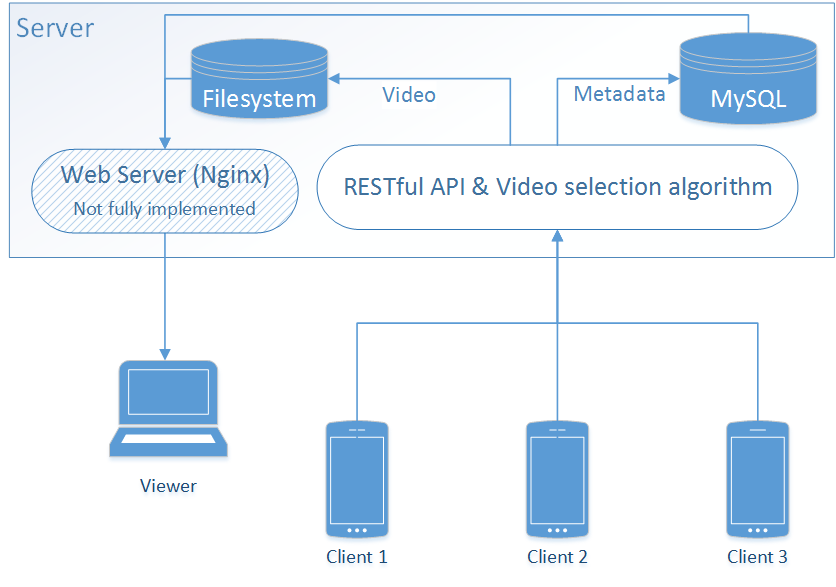
\includegraphics[width=0.45\textwidth]{sys_arch.png}
	%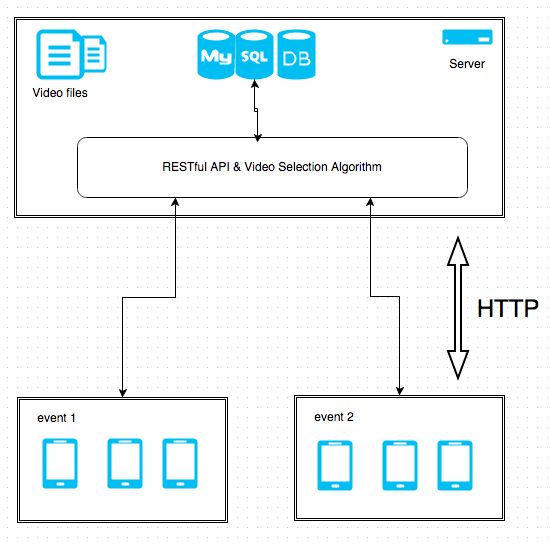
\includegraphics[width=0.45\textwidth]{overview.jpg}
	\caption{General system overview}
	\label{fig:gen_arch}
\end{figure}

\subsection{Client application}

The client application consists of four main logical components: 
user interface, HTTP client, camera and sensor modules and a persistent database.

As a communication protocol between client and server we decided to use HTTP.
Two major options for HTTP clients are Apache HTTP Client and \textsc{HttpURLConnection}.
Since it is recommended to use \textsc{HttpURLConnection} for Android Gingerbread and later \cite{jesse_wilson_androids},
we decided to go with it.
It is lightweight, simple to handle as well as applicable for all purposes we are aiming to do.

In order to ensure a smooth work flow of the application, we have to make use of specific thread techniques.
First it is necessary to prevent network operations blocking the application's user interface, resulting in poor usability experience.
Therefore all network operations need to be run as an instance of the specified \textsc{HttpAsyncTask} class, 
a heredity of the \textsc{AsyncTask} class.
Doing so we make sure that all HTTP requests run asynchronously in the background of the application's main thread.
Secondly, the application requires an automatic upload of selected videos, even when users leave the application.
Such feature can be realized in Android by implementing a service class, which handles background computations in the main thread. 
A second thread within this service class is used to request potential selected video ids via HTTP GET every 10 seconds,
in order to upload video files via HTTP PUT if necessary.
By doing so we make sure, that all network operations run independently and separated of our main thread.

Further core function is the recording of videos. Hereby we do not use the phone's default camera application,
rather writing our own camera activity, which can be suited to our requirements.
Using Android's \textsc{MediaRecorder} class we are able to handle access to the phone's build-in camera
as well as the recording and storage of video files.
Simultaneously sensor data is tracked as well.
In order to couple sensor and video capture we make use of the observer pattern.
Sensor detection classes (\textsc{ShakeDetection} and T\textsc{iltDetetcion}) are implemented as Observables,
while the \textsc{CameraActivity} class registers as a single observer. 
When sensor data changes, the \textsc{CameraActivity} is notified by the observables.
All in all we have decided not to focus on sensor detection and retrieving.
A lot of research has been already done in those parts. Due to the shortage of available time we only retrieve 
some basic accelerometer data, in order to determine the amount of shaking and weight of tilt, 
represented by simple integer values.
The sensor data is part of the meta data which is sent to the server for directing the video upload process.
Hereby the amount of shaking is a counter which is increased by one, when ever shaking is detected.
We assume to be in a shaking motion, when at least two of three accelerometer values have changed related
to their previous values by a specific threshold.
The threshold value is initialized as a float constant with the value 0.7f. This value is exclusively based on experimenting.

In order to keep track and coupling of stored video files and obtained meta data, we make use of a persistent database,
implemented with the lightweight SQLite library, which has support from Android side as well.
The local database set up would not have been entirely necessary. 
But due to simplicity and considerations for future extensions, we decided to have all data in persistence.
Each meta data entry has its unique \textsl{id} and each stored video file has its unique \textsl{filename}.
Therefore we use the database column \textsl{filename} as a unambiguous reference to a specific video file.
When the client gets notified by the server to upload a video, it is necessary to check the filename in the within 
the table entries, selecting the correct file to be uploaded.

\subsection{Server application}

% TODO technologies and structure of server application
% TODO describe all classes and system interactions

The server was created using Java 8, Maven, Spark and Gson. Maven allows simplifies deployment and management of applications,
and spark allows creating RESTful service using Java 8's lambdas, which simplifies client-server interactions.
Gson was used to communicate with clients as well as serialize and deserialize SQL results.

Server application uses a RESTful API to communicate with clients, using actions, such as GET /events.

% TODO
Video storage, database connection, server framework description. RESTful Web Service


\subsection{Client-server interaction}
% TODO BRAINSTROMING: HTTP protocol, 

All client server interaction are carried out using HTTP requests to certain server locations.
Server provides a kind of API which allows client application to upload metadata, query selection results and upload videos.
We decided to use HTTP because it is textual, which means easy to debug, 
wide-spread and well established protocol with a lot of tool already available. 
Another advantage of this protocol is that it does not require to maintain a persistent connection between the two ends.
This important feature allows to prolong battery life and diminish traffic waste.

% TODO ADD DIAGRAM FOR CLIENT-SERVER MESSAGES HERE !!!!!!!!!!!!!!!!!!!!!!!!!!!!!!!!!!!!!!!!!!!!!!!

\subsubsection{Protocols}

Our Automatic Mobile Video Director server implementation provides 
a generalized interface to applications which wish to interact with it. 
It is implemented through RESTful HTTP requests, using certain server locations as actions.

\begin{description}
	\item[GET /events]\hfill\\
		Lists all events (including videos) in~JSON.
		
	\item[GET /event/\textit{id}]\hfill\\
		Returns Event (including videos) in~JSON.
				
	\item[POST /event/new]\hfill\\
		Create new event from JSON.
		Expects request body to be a JSON string containing attribute~\textit{name}.
		
	\item[POST /event/\textit{id}]\hfill\\
		Upload JSON metadata about a video for Event with given \textit{id}.
		
	\item[PUT /video/\textit{video\_id}]\hfill\\
		Upload video~\textit{video\_id} from Event~\textit{id}.
		Expects request body to be a file stream containing a full video file.
		
	\item[GET /video/\textit{video\_id}]\hfill\\
		Retrieve video~\textit{video\_id} from Event~\textit{id}.
		
	\item[GET /selected]\hfill\\
		Retrieve a list of selected but not yet uploaded videos in JSON.	
		
\end{description}

\subsection{Meta data format and exchange}
The exchange of meta data is an important part of our client - server communication.
Therefore it is necessary to define a data interchange format, which fulfills the requirements to describe the meta data properly.
By implementing a RESTful Web Service, two formats are particularly interesting to consider: JSON and XML.
Both formats have their advantages and drawbacks, which are explained in context for our decision making in the following.
%TODO INSERT PAPER Nurzhan Nurseitov + BOOK RICHARSDON & RUBY

JSON is a lightweight and a extremely readable format. Its structural Strings resembles simple data structures in general. 
It is easy to use and parse for computers, which leads to an advantage to save computational power on client and server side. 
Serialization and deserialization between JSON Strings and Objects can be done efficiently, with less effort in comparison to XML.
According to Richardson and Ruby XML is mainly used when it is necessary to describe data structures, which fit into the document paradigm. 
Therefore exchanging meta data in our case does not come with the need to use complex and profound structures like XML. 
Within the HTTP POST REQUEST and HTTP POST RESPONSE, as well as the HTTP GET RESPONSE  of our application, 
the request-/response body can be described as a simple JSON string. In the following all the meta data exchange of our HTTP REQUESTS and 
RESPONSES are shown in the used JSON format:

\begin{description}
	\item[POST /event/\textit{event\_id}]\hfill\\	
				REQUEST: \textit{\{ name:””, finish\_time:””, duration:””, width:””, height:””, shaking:””, tilt:”” \}}\hfill \\
				RESPONSE: \textit{\{ id:””, name:”” \}}

	\item[GET /selected]\hfill\\		
				REQUEST: \textit{\{\}}\hfill \\
				RESPONSE:\textit{\{ id:””, event\_id:””, finish\_ts:””, status:”” \}}

\end{description}

Due to its simple and lightweight character we are able to reduce data traffic between clients and server. 
XML comes with big chunks of data in raw text format, which makes the size overhead in comparison to JSON crucial.
The data traffic amount might seem not differ much at first, but considering that a plurality of clients request GET/selected every 10 seconds and upload videos via the mobile network, client costs and bandwidth problems are definitely minimized using JSON. Therefore we decide to use JSON as our preferred interchange format language.

Meta data describes the characteristics of recorded videos. Its main attributes, already shown above in JSON, are:

\begin{description}
	\item[id] 
		Server-side unique identification of the video. 
		On Client side named as server\_id and transferred from server to client in the POST RESPONSE.
		
	\item[name]
		File name in client's local file system.
		
	\item[finish\_time]\hfill\\
		Video creation time.
		%TODO Is it really so?
		
	\item[duration]\hfill\\
		Video duration.
		%TODO This thing too.
		
	\item[width]\hfill\\
		Video frame width in pixels.

	\item[height]\hfill\\
		Video frame height in pixels.		
	
	\item[shaking]\hfill\\
		Amount of shaking detected by sensors.

	\item[tilt]\hfill\\
		The amount of tilt holding of the camera.
	
	\item[status]\hfill\\
		Video status. Indicates video life cycle phase.
		% TODO It would be nice to decide on video lifecycle both client- and server-side.
		%	It would make a nice diagram to include in the report.

		
\end{description}

\section{Video Director Algorithm}

\subsection{Video life cycle}

Video metadata is stored in the database upon receiving it from a client. A temporary video instance
is then created on the server to manage interactions with a short-lived client session. Once that session
is over, the client will no longer be able to upload his videos, unless he uploads the same metadata again.
The server would likely not accept these new videos as a great deal of time would have passed. Any live stream
would be running far ahead of the time these videos were shot. After the client has uploaded metadata, the
videos are store in the database with the status flag set to 0 (METADATA). To be able to upload a video,
the client must connect to the server, and issue a HTTP GET call on /selected, where the server will make
a decision on which videos of his that will be eligible for upload. If a video is selected, identifying
information is returned as a JSON string, and the client can then issue HTTP POST with path /video/[id].
Once the video has been received, its status is set to 1 (RECEIVED). A video can further be promoted to
status 2 (PUBLISHED), in which it could be visible for, say, an event stream.

Due to many videos not being actively uploaded, and older videos still remaining, a pruning mechanism could
be implemented to clean out older videos and metadata.

\subsection{Selection algorithm}

When selecting a video for upload, the server will consider all pending videos for a given client,
then for each event of a video (should be just one) check if the client has any pending videos that
are top-ranked. This is done through a simplistic ranking algorithm that considers video duration, tilt
and shaking. The latter two based on motion sensor data. Tilt and shaking is mapped from 0 to infinity
using a sigmoid function separately, and then transformed to account for video duration. The last step
is weighing tilt and shake (with duration accounted for) and then scaling it from 0-100.
The selection algorithm is currently calibrated to work best with shorter videos ranging from 10-60 seconds,
although it may at any point be recalibrated for any other arbitrary range.

EXPAND FURTHER.

\section{Evaluation}
How good/bad it is.

\subsection{Data Traffic} 
Thilo can test it. I will have a look to this. If someone has experience please let me know.

1. Measure data consumption
2. Find data from other video streaming service
3. Comparison

\subsection{Selection criteria}

Describe the algorithm we use now
1. We assign some rating based on metadata
2. We select video based on where the event is at, based on video timestamps
etc.

\section{Future Work}

Our implementation is far from perfect, especially compared to similar existing systems.
This is due to the fact that our system was implemented in five weeks and 
we did not have time to include all the features that could have been in such a system.
Among the things which could be improved are a better way of identifying a timeline of an event,
a way of identifying regions of interest, real-time streaming from mobile devices to server 
and from server to end users with minimum delay, web portal to navigate covered events and many more.
In this section we will go through these points, look at the problems we encounter with our solution 
and suggest better implementation alternatives where available.

The timestamps represent a weakness in our system.
They are generated based on the clock in the mobile device which is not necessarily accurate or 
synchronized to server time or even timezone. 
This creates uncertainty about the actual time a video was captured as it relies on us trusting the devices all have the exact same time.
This is practically impossible as the system is intended for use by general public. 
There are two ways presented in the sources for this paper for solving this. 
\cite{shrestha_automatic_2010} presents a system that uses the audio of a video file to pinpoint the duration of an event it covers.
It does this by comparing audio to other video files looking for what they call “audio-fingerprints”. 
According to them, it is a robust method that calculates the time offset of a video in about 11.6 ms. 
Another way is just mentioned in \cite{ jain_focus:_2013} and uses the GPS device located on a mobile device
to generate what they call “precise GPS-derived timestamps”.
Either of these methods would be better than ours as they don’t rely on what time is set on the users device,
however, we deemed them very time-consuming to implement, and so decided to implement them only if we had time for it.
We are fully aware of possible errors our current methods might cause.

Region of interest is a very interesting topic in this field as it focuses on making sure 
that the right content is captured during an event.
The fact that we do not have it implemented has a few implications to the practical use of our system.
First of all, we cannot be sure what is shown on the video. 
We do not check where the mobile device is when it films so the person filming may not be at a listed event at all.
We can solve this by checking the users GPS when they try to connect to our server, or when they deliver a video file.
When creating an event we would have to mark up the coordinates where the event is taking place 
and only accept videos delivered from within the designated area.
Even if we make sure the person is at the event we cannot be sure he or she is pointing the camera in the right direction.
This problem can be solved by checking the built-in compass in the mobile device 
and only accepting videos that are shot in the right direction, as proposed in \cite{cricri_sensor-based_2012}.
So if we want to film a concert we only accept files from clients that are at the event and are pointing their camera at the stage. 
Identifying where the videos are shot and what they show is also impacted by issues of privacy and commercial interests. 
With our system we can shoot videos anywhere, at any time, but this can come in conflict with legal rights 
if we use the application to film a person without their consent.
We would also come in conflict with TV-channels, sitting on the rights for covering a sports event, 
if we use our system to provide a free alternative to theirs, without their permission. 
Making sure the system can properly identify the regions of interest is therefore very important.

When we talk about multimedia system, one of the most important results is delivered content. 
While we do implement some limited streaming capabilities, a proper web portal, which allows to choose an event 
and see the stream right from a browser, would be a logical final to video's path through out system.
It is not hard to implement, but it needs time and some basic web programming knowledge which is quite different from our other tasks.

\section{Conclusion}
The conclusion goes here.

% TODO
WRITE ME:
EXAMPLE:
We built a system with video selection algorithm using metadata from clients and so on.
What did we achieve?


% trigger a \newpage just before the given reference
% number - used to balance the columns on the last page
% adjust value as needed - may need to be readjusted if
% the document is modified later
%\IEEEtriggeratref{8}
% The "triggered" command can be changed if desired:
%\IEEEtriggercmd{\enlargethispage{-5in}}

% trigger a \newpage just before the given reference
% number - used to balance the columns on the last page
% adjust value as needed - may need to be readjusted if
% the document is modified later
%\IEEEtriggeratref{8}
% The "triggered" command can be changed if desired:
%\IEEEtriggercmd{\enlargethispage{-5in}}

% references section

% can use a bibliography generated by BibTeX as a .bbl file
% BibTeX documentation can be easily obtained at:
% http://www.ctan.org/tex-archive/biblio/bibtex/contrib/doc/
% The IEEEtran BibTeX style support page is at:
% http://www.michaelshell.org/tex/ieeetran/bibtex/
\bibliographystyle{IEEEtran}
\bibliography{report}
% argument is your BibTeX string definitions and bibliography database(s)
%\bibliography{IEEEabrv,../bib/paper}

%\newpage

\begin{table*}[t]
	\centering
	\renewcommand{\arraystretch}{1.5}
	\caption{Task distribution}
	\label{tab:task_distr}
	\begin{tabular}{lllr}
		\toprule
		Part & Task & Subtask & Responsible \\
		\midrule
		Design
			& Server application & & Alf-André Walla \\
			& Client application & & Thilo Weigold \\
			& Client-server interactions & & Alexander Egurnov, Alf-André Walla \\
		\midrule
		Android application
			& Video Capture & Implementation & Thilo Weigold \\
			&       & Autofocus & Alexander Egurnov \\
			& MediaManager & & Thilo Weigold \\
			& Sensor data collection & & Thilo Weigold \\
			& Metadata class & & Thilo Weigold \\
			& Http Client & Post Method & Thilo Weigold \\
			&       & Cookies, Callbacks & Alexander Egurnov \\
			&       & Get \& Upload methods & Alexander Egurnov \\
			& Background upload service & & Thilo Weigold \\
			& SQLite database connection & & Thilo Weigold \\
			& Preferences & & Alexander Egurnov \\
			& GUI & & Thilo Weigold, Alexander Egurnov \\
			& Client-server data exchange & & Alexander Egurnov \\
		\midrule
		Server application 
			& RESTful Server application & Client authorization & Alf-André Walla \\
			&       & Request processing & Alf-André Walla \\
			&       & Video and Event logic & Alf-André Walla \\
			& MySQL database connection & & Jon Pettersen \\
			& Video Director & & Alf-André Walla \\
			& Client-server data exchange debug & & Alexander Egurnov \\
			& Video upload & & Alf-André Walla, Alexander Egurnov \\
		\midrule
		Evaluation
			& Data usage & & \\
		\midrule
		Web Server
			& MySQL Administration & & Alexander Egurnov \\
			& Nginx setup for streaming video & & Alexander Egurnov \\
		\midrule
		Documentation 
			& Basic template formatting & & Alexander Egurnov \\
			& General editing & & Alexander Egurnov \\
			& Images and other data & & Thilo Weigold, Alexander Egurnov \\
			& Introduction & & Thilo Weigold, Alexander Egurnov \\
			& Related Work & & Jon Pettersen, Alexander Egurnov \\
			& Methodology & System Overview & Thilo Weigold \\
			&		& Client application & Thilo Weigold \\
			&		& Server application & Alf-André Walla, Jon Pettersen \\
			&		& Client-server interactions & Alexander Egurnov \\
			& Video Director & & Alf-André Walla \\
			& Evaluation & & \\
			& Future Work & & Jon Pettersen \\
			& Conclusion & & \\
		\bottomrule
    \end{tabular}%
\end{table*}%

\vfill

\end{document}
